\documentclass[11pt]{article}
\usepackage{amsthm,amsfonts,amssymb,amsmath}
\usepackage{tikz}
\usetikzlibrary{positioning}
% Optional PGF libraries
\usepackage{pgflibraryarrows}
\usepackage{pgflibrarysnakes}
\usepackage[top=1in, bottom=1in, left=1.25in, right=1.25in]{geometry}
\usepackage{enumerate}
\usepackage[colorlinks,linkcolor = black, anchorcolor = black,citecolor = black]{hyperref}

\author{Zihao Wang\footnote{N-number: N11385738, NetID: zw1074}
	}
\title{\textbf{Solution for Problem Set 1}}

\begin{document}

\maketitle
\section*{Problem 1}
This problem states a scheduling problem whose goal is to find out a schedule that can make processor get at least target value $ M $ by the deadline $ D $. 

To illustrate this problem, I would like to give an example ($ D = 7 $, $ M = 12 $). (It is the example given in Problem 1) 

\begin{center}
	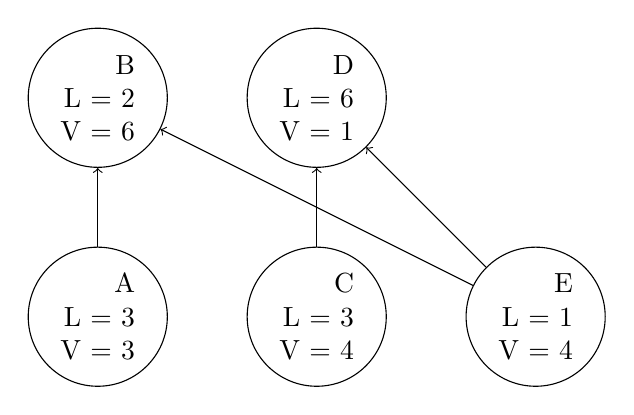
\begin{tikzpicture}
		\tikzset{Task/.style = {circle, draw,align = right}}
		\node[Task]    (B)                {B \\ L = 2\\ V = 6};
		\node[Task]    (D) [right = of B] {D \\ L = 6\\ V = 1};
		\node[Task]    (A) [below = of B] {A \\ L = 3\\ V = 3};
		\node[Task]    (C) [right = of A] {C \\ L = 3\\ V = 4};
		\node[Task]    (E) [right = of C] {E \\ L = 1\\ V = 4};
		\draw [->] (A) -- (B);
		\draw [->] (C) -- (D);
		\draw [->] (E) -- (B);
		\draw [->] (E)  -- (D);
	\end{tikzpicture}
\end{center}

This example can be solved by both BFS and DFS. All of these methods are based on a tree-structured state space. I would like to draw level 1 to 3 of the tree.

\begin{center}
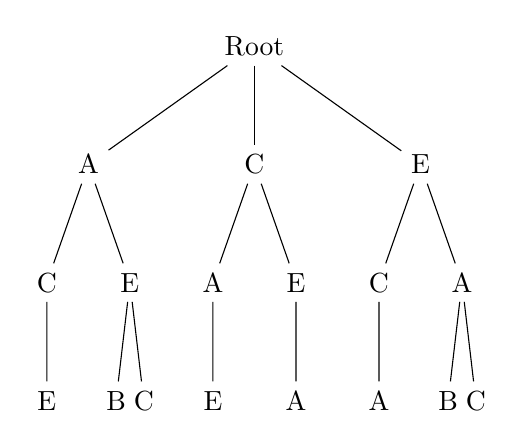
\begin{tikzpicture}[level 1/.style={sibling distance=6em}, level 2/.style={sibling distance=3em},level 3/.style={sibling distance=1em}]

  \node {Root}
    child {node {A}
    	child {node {C}
    		child {node {E}}}
    	child {node {E}
    		child {node {B}}
    		child {node {C}}}
    }
    child {node {C}
      child {node {A}
      	child {node {E}}}
      child {node {E}
      	child {node {A}}}
    }
    child {node {E}
    	child {node {C}
    		child {node {A}}}
    	child {node {A}
    		child {node {B}}
    		child {node {C}}}
    };
\end{tikzpicture}
\end{center}

From this tree, I can get:
\begin{itemize}
	\item \textbf{States}: All possible arrangement of tasks (not allow to repeat) that their total time will not exceed the deadline.
	\item \textbf{Initial State}: Any tasks that no other tasks point to.
	\item \textbf{Operators}: Add any task that meet the requirement 'not exceed the deadline.'
	\item \textbf{Branching Factor}: The number of any other available tasks.
	\item \textbf{Goal Test}: Is the total value of the tasks array not less than target value.
	\item \textbf{The Depth of Goal}: Because the value and execute time of each task may be different, the depth of the goal is not known initially.
\end{itemize}

However, even if we don't know the depth $ d $ of the goal, we can still know the upper bound of the value (if it exits). It is $ d\leq \min(N,[M/X] + 1,[D/Y]) $. $ X = \min_{T}T.V $, the smallest value, and $ Y = \min_{T}T.L $, the smallest time requirement. ($ [x] $ is the greatest integer that is not greater than $ x $.)
\begin{proof}
	We just need to prove  $ d $ is not greater than any value of $ (N,[M/X] + 1,[D/Y]) $.
	
	As to $ N $,clearly, because the tasks can not be executed repeatedly, the task number of any possible array will not greater than $ N $. So $ d\geq N $.
	
	As to $ [M/X] + 1 $, supposed that there exists a goal that its depth $ d $ is greater than $ [M/X] + 1 $ and it can be written as $ (a_1,a_2,\dots,a_d),~d\leq N $. Then, we have $$ \sum_{i=1}^{d-1}a_i.V<M. $$ Because if this list does not have this property, it can be shortened. From $ a_i.V\geq X $, we have $$ M>\sum_{i=1}^{d-1}a_i.V\geq (d-1)X. $$ Therefore, we have 
	\begin{align*}
		d< \frac{M}{X} + 1.
	\end{align*}
	However, from the assuming, we know that $ d>[M/X] + 1 $. And because $ d $ is an integer, we can know $$ d\geq \left[\frac{M}{X}\right] + 2. $$ From the definition of $ [\cdot] $, we also have $ x - [x] < 1 $. So $$ d>\frac{M}{X} + 1. $$It leads to contradiction, so $ d\leq [M/X] + 1 $.
	
	As to $ [D/Y] $, without loss of generality, assumed a 'successful' tasks arrangement can be written as $ (a_1,a_2,\dots,a_d) $, we can have $$ dY\leq\sum_{i=1}^{d}a_d.L\leq D. $$ So $ d\leq D/Y, $ and because $ d $ is an integer, we also have $$ d\leq [D/Y]. $$
\end{proof}

\section*{Problem 2}
Using the tree-structured state space in \textbf{Problem 1}, the portion of DFS is:

\begin{center}
	\begin{tikzpicture}[level 1/.style={sibling distance=6em}, level 2/.style={sibling distance=3em},level 3/.style={sibling distance=1em}]
	
	\node {Root}
	child {node {A}
		child {node {E}
			child {node {B}}
			}
	}
	child {node {C}}
	child {node {E}};
	\end{tikzpicture}
\end{center}

And as to BFS:
\begin{center}
	\begin{tikzpicture}[level 1/.style={sibling distance=6em}, level 2/.style={sibling distance=3em},level 3/.style={sibling distance=1em}]
	
	\node {Root}
	child {node {A}
		child {node {C}
			child {node {E}}}
		child {node {E}
			child {node {B}}
			}
	}
	child {node {C}
		child {node {A}
			}
		child {node {E}
			}
	}
	child {node {E}
		child {node {C}
			}
		child {node {A}
			}
	};
	\end{tikzpicture}
\end{center}

\section*{Problem 3}
\subsection*{A}
\begin{center}
	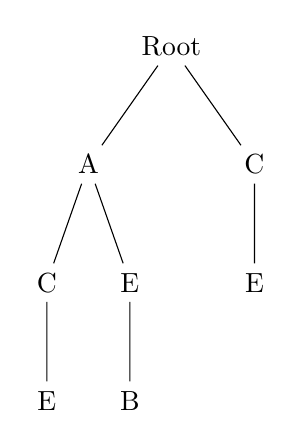
\begin{tikzpicture}[level 1/.style={sibling distance=6em}, level 2/.style={sibling distance=3em},level 3/.style={sibling distance=1em}]
	
	\node {Root}
	child {node {A}
		child {node {C}
			child {node {E}}}
		child {node {E}
			child {node {B}}
		}
	}
	child {node {C}
		child {node {E}
		}
	};
	\end{tikzpicture}
\end{center}
\subsection*{B}
Using a hash table would be a useful method to eliminate repeated states. To construct a hash table, hash function is necessary. The hash function I choose is a $ N $-digit binary array. The position of each '1' represents the task I select. Therefore, for example, $ f(\mbox{'AC'}) $ in the example in \textbf{Problem 1} will be '10100', which is the same as $ f(\mbox{'CA'}) $. To implement this function to BFS method, the node should be changed to the value of hash table. And this will reduce much repetition.

Again, the key of this function is the arrangement of tasks' ID. Then use the number 1 to $ N $ to represent each task. So the value of this function is which tasks are selected, and then transfer to 1 in corresponding position in a $ N $-digit binary array. (e.g. $ f(\mbox{'ABC'}) = 11100,f(\mbox{'AD'}) = 10010 $)

Then during searching, we may add a new binary array when we have a new arrangement without considering permutation.
\subsection*{C}
The hash table is definitely useful in BFS because BFS will check every $ k $-long arrangement of task ($ k<d $, where $ d $ is the depth of goal node), so by using hash table to eliminate repetition, this will reduce by about $ \sum_{i=1}^{k}i! $ memory to store the arrangement. And once we get a correct return, it is very easy to find out the true sequence of task.

However, to DFS, it is not very useful. Because DFS will dig the depth first and the memory it uses is just $ N $, so there is no need to create another $ 2^N $ space to store the binary array.

And also to iterative deepening, it use DFS locally, so it is the same reason as DFS.
\subsection*{D}
To eliminate the repetition and meanwhile apply the advantage of DFS or ID algorithm (low memory required), we can construct a sort from the DAG. And that is called topological sort.

\textbf{Definition\footnote{Detail can be refered to \url{https://en.wikipedia.org/wiki/Topological_sorting}.}}: A sort that is called topological sort is a linear ordering of its vertices such that for every directed edge uv from vertex u to vertex v, u comes before v in the ordering.

Due to the construction of DAG (the generating algorithm in \textbf{Programming Assignment 1}\footnote{Experiment on \url{http://cs.nyu.edu/courses/fall15/CSCI-GA.2560-001/prog1.html}}), it must be a directed acyclic graph. So we could find out a topological sort in every connected vertex according to \textbf{Zorn's lemma}\footnote{More details can be found on \url{https://en.wikipedia.org/wiki/Zorn\%27s_lemma}}
. Then, we can distribute the DAG into several subsets. And the subsets will have only two types. One is that every point in it is connected, then we can find out a topological sort from it. The other one is that every point in it is a single point, which is not connected to any other point.

So we can get a sort from type 1 and express it as $ \lbrace a_1,a_2,\dots,a_k \rbrace $. The pre-finish task of $ a_i $ in this sort must be some tasks $ a_j $ that $ j<i $. And because different type 1 subsets are not connected, so we can combine then by any order. So we can have a new sort for all type 1 subsets' points $ \lbrace b_1,b_2,\dots,b_m \rbrace $. And then we can just need to add type 2 points on the front of the list. So we can have a new list for all points in DAG $ S = \lbrace c_1, c_2,\dots, c_N\rbrace $.

When we add a new node by using ID and DFS algorithm, we can first check if this node $ a_j $ is after the parent node $ a_i $. If it is so and follows the rule of the tasks, we can add it as a child node. Because every node must follow the subscript order of $ S $, we eliminate the repetition.
\end{document}

